\documentclass[11pt, a4paper]{report}
\usepackage[utf8]{inputenc}%codification of the document
\usepackage[french]{babel}
\usepackage{geometry}
\usepackage{times}
\usepackage{graphicx}
\usepackage{multicol}
\usepackage{float}
\usepackage{subcaption}
\usepackage{comment}
\usepackage{hyperref}
\usepackage{listings}
\usepackage{color}

\definecolor{lightgray}{rgb}{.98,.98,.98}
\definecolor{darkgray}{rgb}{.4,.4,.4}
\definecolor{blue}{rgb}{0.5, 0.2, 0.82}
\definecolor{purple}{rgb}{0.7, 0, 0.6}

\lstdefinelanguage{JavaScript}{
	keywords={typeof, new, true, false, catch, function, return, null, catch, switch, var, if, in, while, do, else, case, break},
	keywordstyle=\color{blue}\bfseries,
	ndkeywords={class, export, boolean, throw, implements, import, this},
	ndkeywordstyle=\color{darkgray}\bfseries,
	identifierstyle=\color{black},
	sensitive=false,
	comment=[l]{//},
	morecomment=[s]{/*}{*/},
	commentstyle=\color{blue}\ttfamily,
	stringstyle=\color{purple}\ttfamily,
	morestring=[b]',
	morestring=[b]"
}

\lstset{
	language=JavaScript,
	backgroundcolor=\color{lightgray},
	extendedchars=true,
	basicstyle=\footnotesize\ttfamily,
	showstringspaces=false,
	showspaces=false,
	numbers=left,
	numberstyle=\footnotesize,
	numbersep=9pt,
	tabsize=2,
	breaklines=true,
	showtabs=false,
	captionpos=b
}



\begin{document}
	\pagenumbering{roman}
	\begin{titlepage}
		\begin{center}
			
			\vspace*{1cm}
			
			\begin{figure}[h]
				\centering
				
\includegraphics[width=0.4\textwidth]{images/LOGO_Polytech-lille.jpg}
				\hspace{2cm}
				
\includegraphics[width=0.4\textwidth]{images/logo_ulille_transparent.png}
			\end{figure}
			
			\vspace*{2cm}
			
			\rule{1\textwidth}{.8pt}
			
			\LARGE{\textsc{Projet tutoré de Structures de Données \\-\\ Graphes et Combinatoires}}
			
			\vspace*{1cm}
			
			\LARGE{\textsc{Problème du flot maximum}}
			\vspace*{1cm}
			
			\small{IS2A3 - Lundi 31 mai 2021}
			
			\vspace*{0.5cm}
			\rule{1\textwidth}{.10pt}
		
			\vspace*{2.352cm}
			
			\large{\textit{Encadrante :} Clarisse DHAENENS}
			
			\vspace*{0.1cm}	        
			
			\large{\textit{Auteurs :} Badmavasan KIROUCHENASSAMY\\Caroline SCHMID} 
			
			
			
			
		\end{center}
		
	\end{titlepage}
	
	
	%\setcounter{tocdepth}{2}
	\tableofcontents
	
	
	\chapter{Contexte du projet}
	\pagenumbering{arabic}
	Pour résoudre un problème de flot maximum, plusieurs algorithmes peuvent être mis en œuvre. Nous étudions ici la mise en place de l'algorithme de \textbf{DINIC} ainsi que les structures de données nécessaires et l'arborescence des fichiers.
	
	Le problème de flot maximum consiste en trouver le flot le plus élevé que l'on puisse faire passer dans un Réseau en respectant les capacités de chaque arc, soit le flot maximum que l'on puisse faire passer par chaque arc.
	
	L'algorithme de \textbf{DINIC} permet, à partir d'un flot initial, de rechercher une chaîne améliorante dans un réseau de façon à construire un flot de valeur supérieure. En réitérant cette opération un certain nombre de fois, le flot que l'on obtient devient maximum. L'algrithme prend en paramètre un graphe d'écart, il faut donc trnsformer le réseau du problème de flot maximum en un graphe d'écart pour trouver le flot maximum et revenir à un réseau répondant au problème posé.
	
	On considère que le flot initial est de 0 et que les sommets sont au nombre de $n$ et numérotés de $1$ à $n$.
	
	
	
	\chapter{Analyse}
	La chaîne améliorante de l'algorithme de \textbf{DINIC} est la chaine du plus court chemin en nombre d'arcs et sera trouvée donc par l'algorithme de parcours en largeur. Étant donné que ce dernier algorithme génère l'arborescence donnant le plus court chemin en nombre d'arc, on l'utilise pour trouver la chaîne améliorante de l'algorithme de \textbf{DINIC}.
	
	L’algorithme de parcours en largeur est un algorithme parcourant le graphe par couches. Les sommets de la couche $n$ sont à une distance $n$ du sommet source. L’exploration commence donc par la source, puis ses successeurs, puis les successeurs de ses successeurs, ... jusqu’à explorer le sommet puits et on sait alors que l’on peut s’arrêter. Grâce à un tableau répertoriant les prédécesseurs des sommets marqués (par convention, le sommet prédécesseur du sommet source est lui-même), on peut retrouver le chemin le plus court en nombre d'arcs menant d’un sommet à un autre (ici, menant du sommet source au sommet puits).
	
	Voici le déroulement de l'algorithme de \textbf{DINIC} sur un réseau à 5 sommets et 7 arcs :
	\begin{enumerate}
		\item \verb|Réseau :|\\
	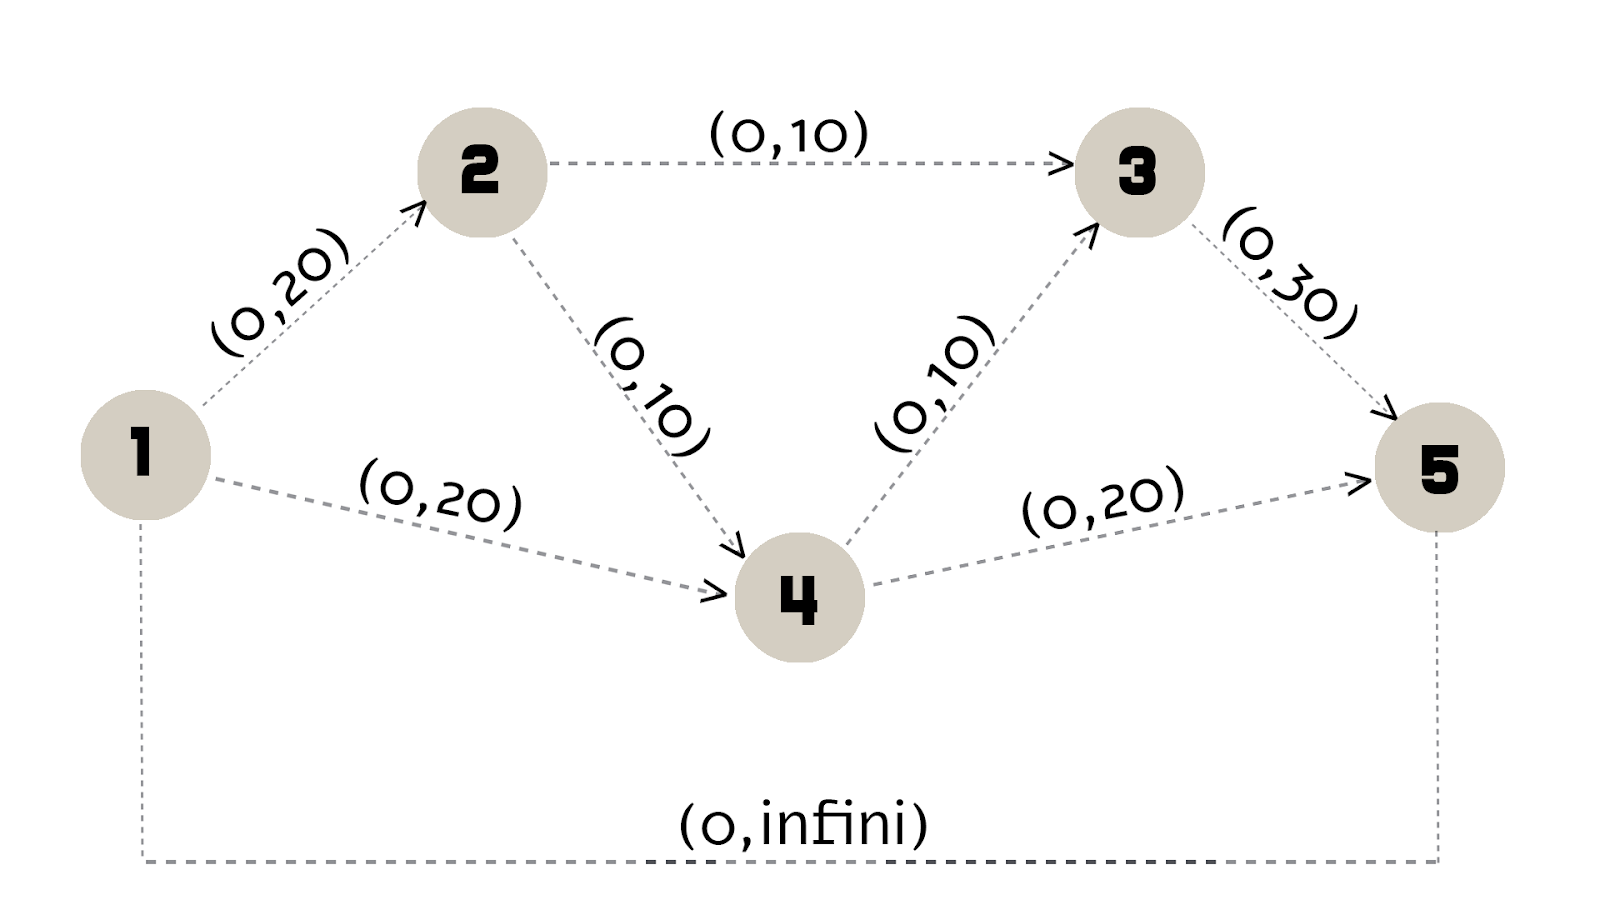
\includegraphics[width=0.7\textwidth]{images/R1.png}\\
	\pagebreak
		\item \verb|Graphe d'Écart :|\\
	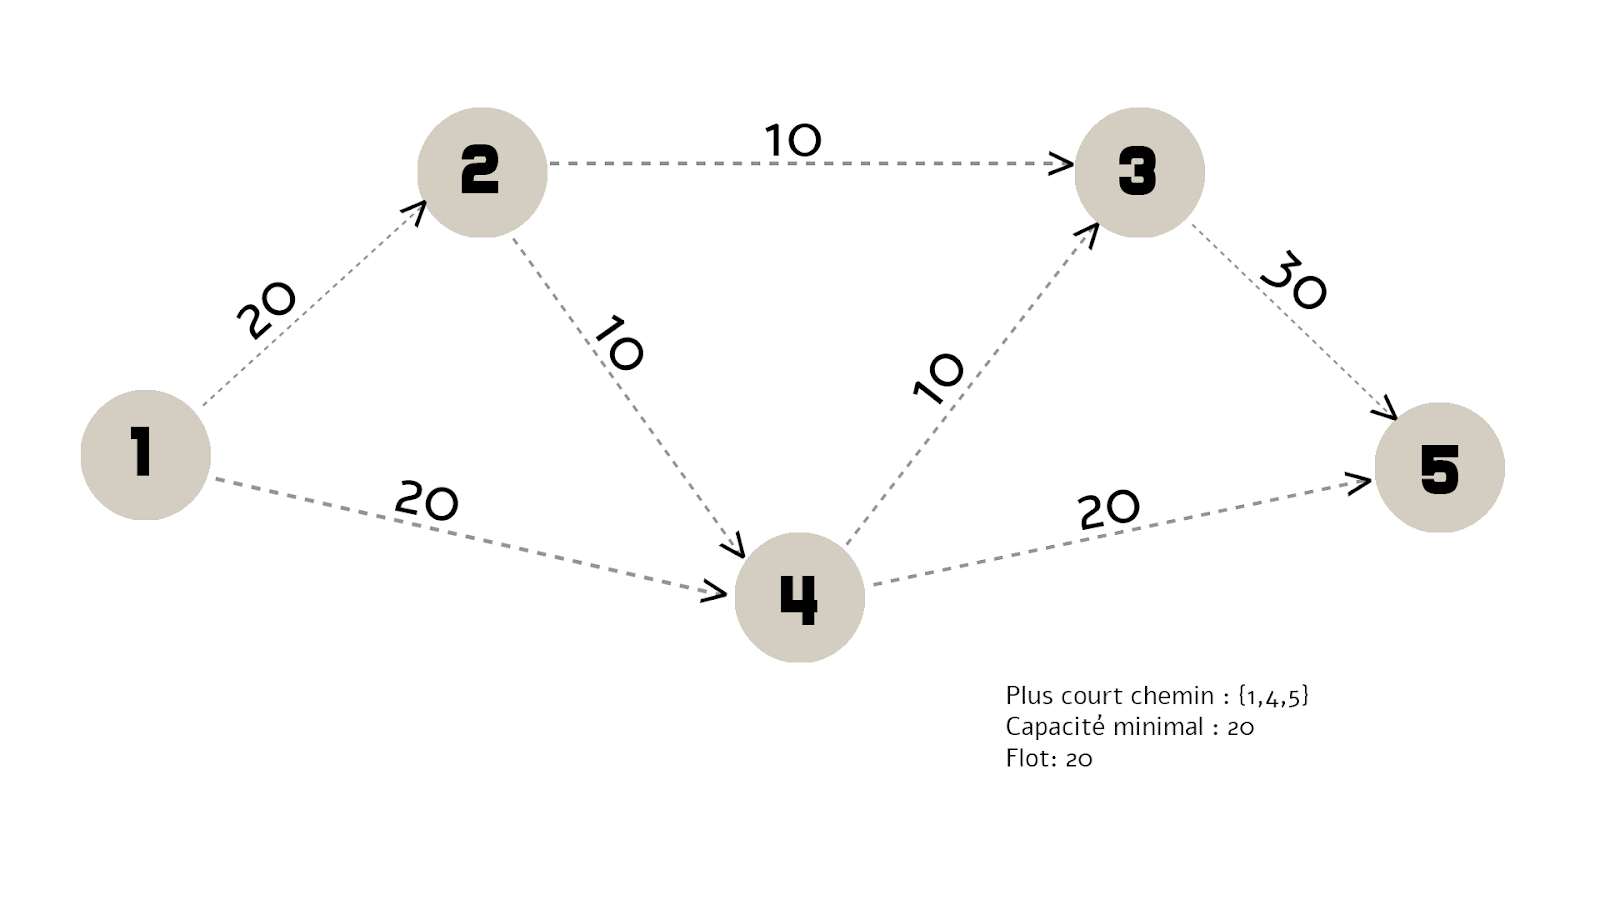
\includegraphics[width=0.7\textwidth]{images/GE1.png}\\
		\item \verb|Graphe d'Écart :|\\
	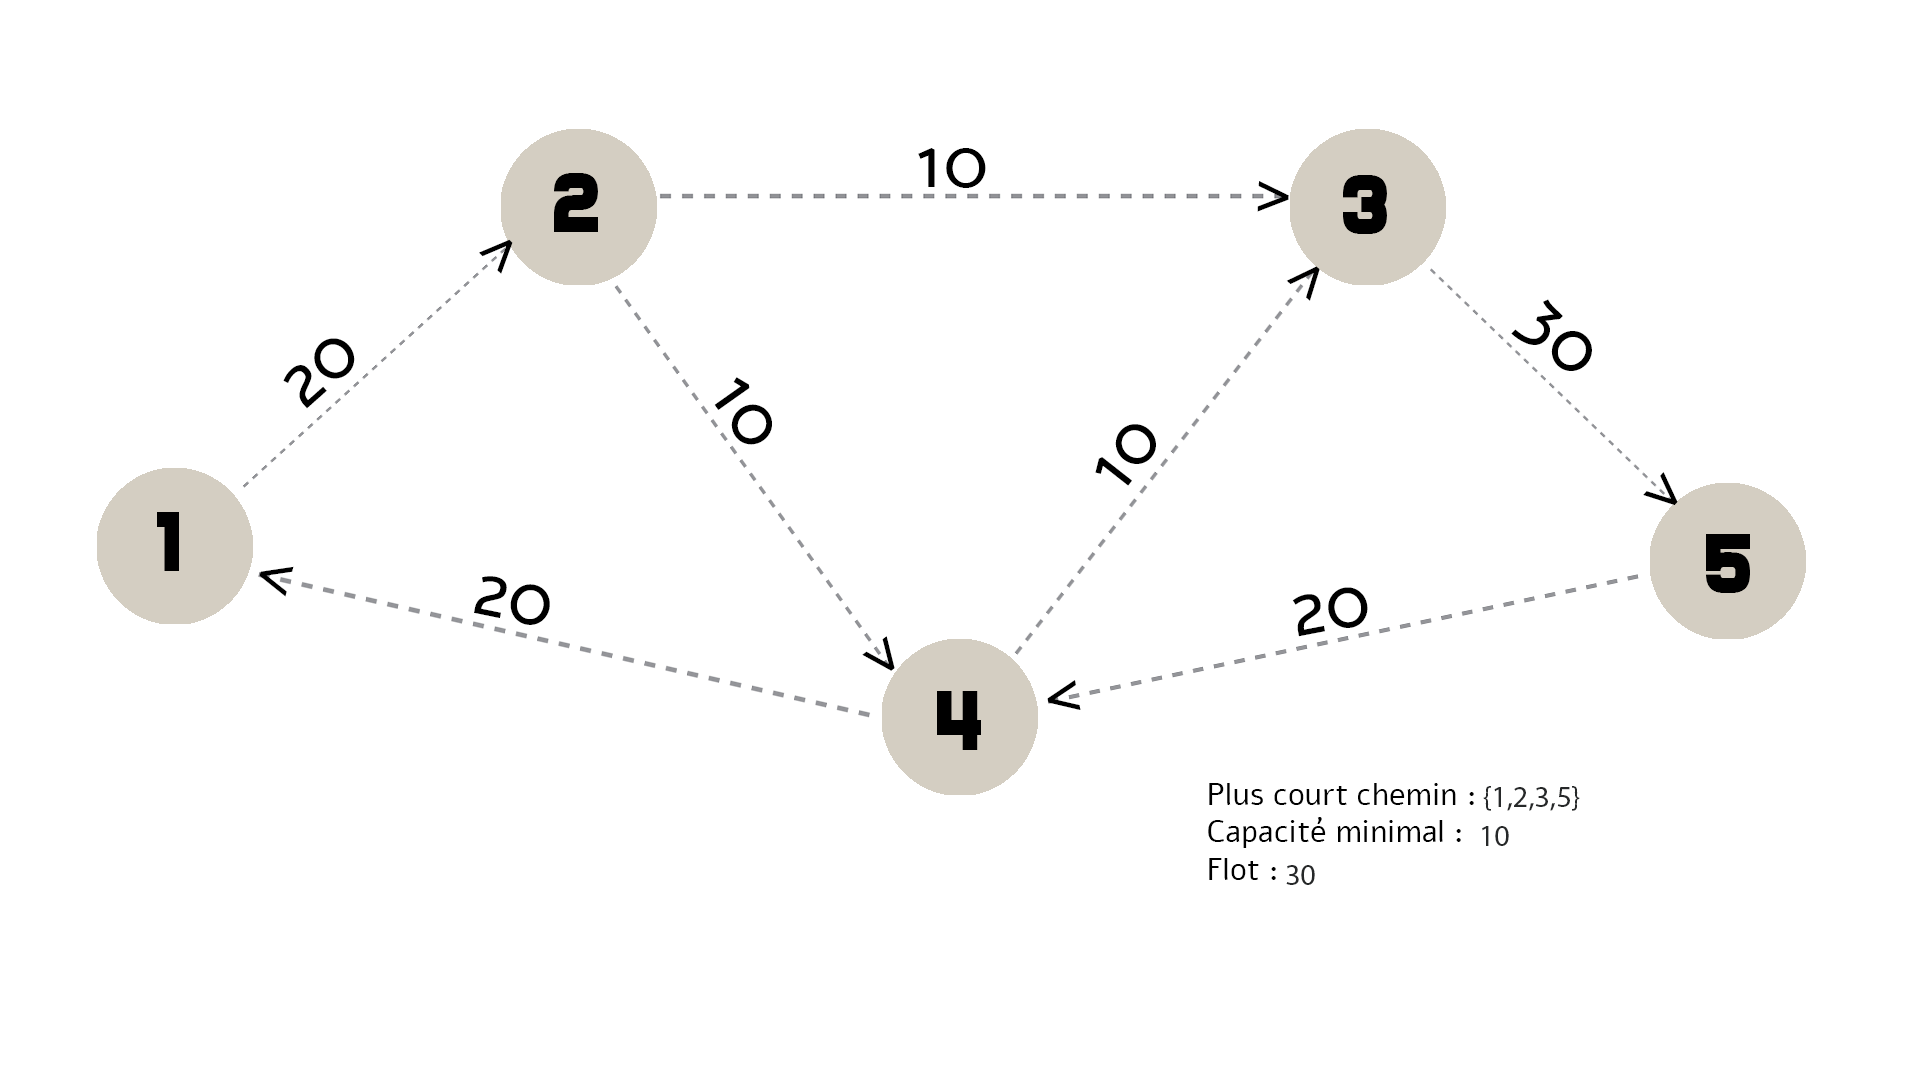
\includegraphics[width=0.7\textwidth]{images/GE2.png}\\
		\item \verb|Graphe d'Écart :|\\
	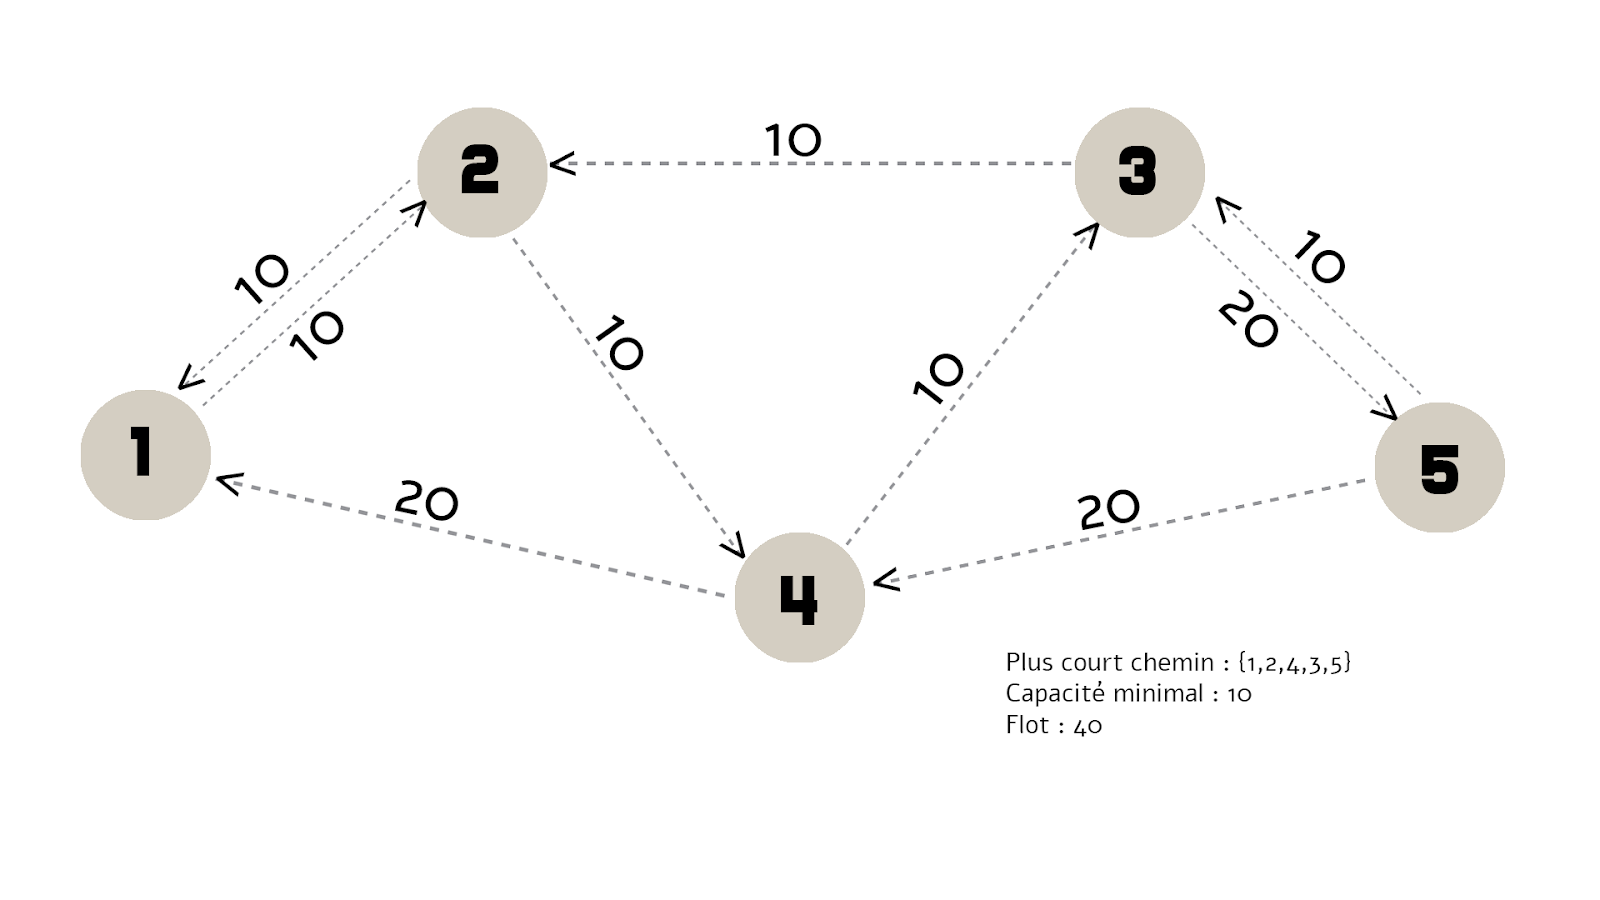
\includegraphics[width=0.7\textwidth]{images/GE3.png}\\
	\pagebreak
		\item \verb|Graphe d'Écart :|\\
	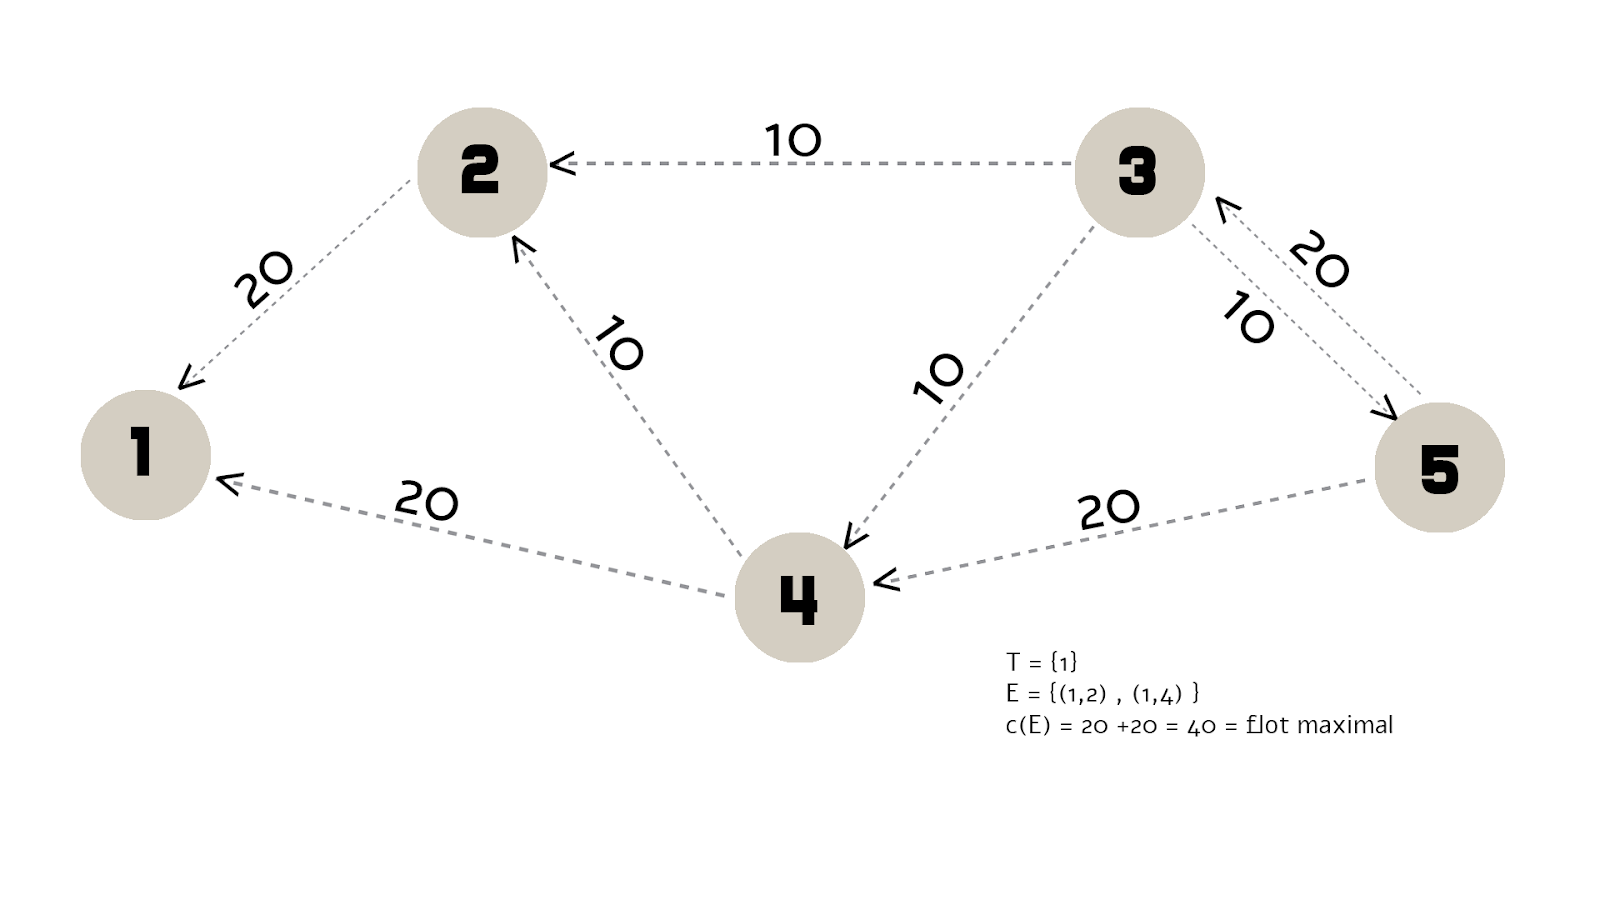
\includegraphics[width=0.7\textwidth]{images/GE4.png}\\
		\item \verb|Réseau :|\\
	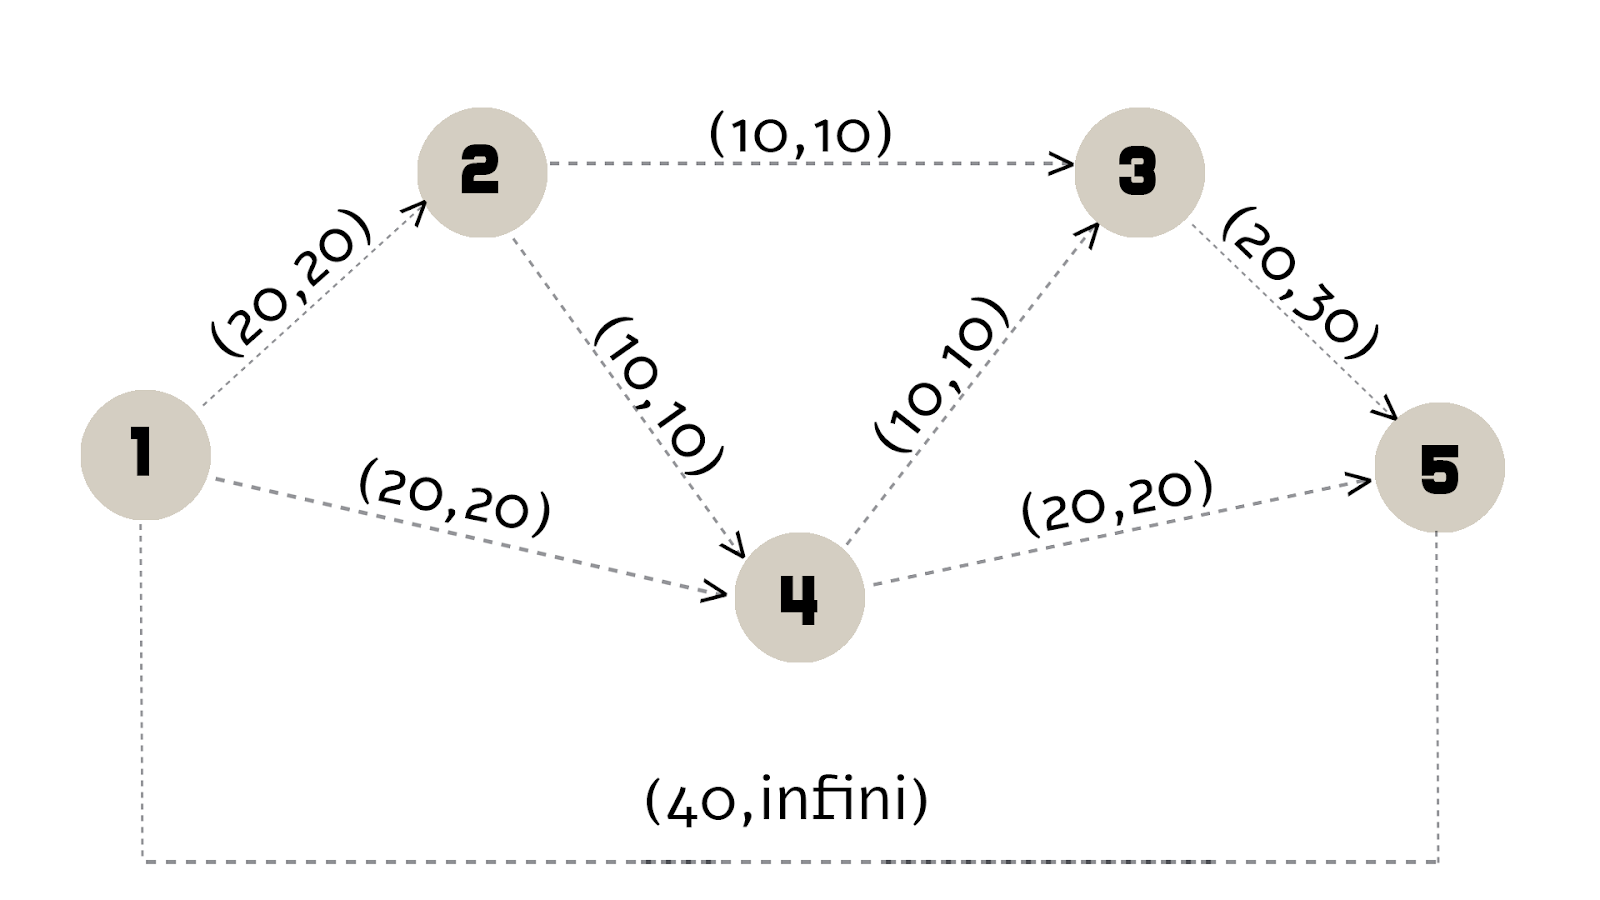
\includegraphics[width=0.7\textwidth]{images/R2.png}\\
	\end{enumerate}
	
	
	
	\chapter{Mode d'emploi}
	Le matériel utilisé à été les différentes banques de polymères et de monomères ; les méthodes utilisées ont été les deux programmes.
	
	%\section{Matériel}
	Les banques de données sont Norine et PubChem. PubChem est la banque de données américaine. Les données de ces deux banques sont représentées au format Smiles. Le Smiles est un langage de description de la structure atomique des monomères et polymères, utilisé en chémo-informatique. Un nouveau format est en cours de création : le format HELM. HELM reprend la notation Smiles et l'enrichit d'informations comme l'emplacement des liaisons peptidiques, qui est le lieu où deux monomères s'assemblent.
		
	Dans un premier temps, pour apprendre à manier et maîtriser Smiles2 Monomers et rBAN, j'ai utilisé la banque de monomères et de polymères de Norine. Pour ce faire, j'ai téléchargé les deux banques au début de chaque jour, les ai mises en forme pour n'en garder que le nécessaire et les ai placées en entrée des programmes.
	
	L'étape suivante à été l'utilisation de la banque de polymères de PubChem. Dans un premier temps, j'ai téléchargé un fichier de 500'000 identifiants de polymères et leur Smiles associés. Grâce à l'identifiant, j'ai pu télécharger la fiche descriptive de chaque polymères pour y récupérer le nom de celui-ci. Smiles2Monomers déclenchait cependant une erreur lorsque le nom du polymère était trop long. Il a donc été décidé de remplacer le nom par l'identifiant (de 9 caractères) et de créer un fichier $.html$ permettant de faire le lien entre l'identifiant et la description du polymère. Ceci permet également de ne plus télécharger les descriptions des polymères en début de chaque lancement des programmes et de tout faire à partir du fichier d'identifiants-Smiles.
	
	La dernière étape a été de remplacer les monomères venant de Norine par ceux de HELM, que ma responsable Madame Pupin m'a transmis en deux fichiers et dont j'ai extrait l'utile et mis en forme pour que Smiles2Monomers et rBAN l'accèptent.
	
	%\section{Méthodes}
	Smiles2Monomers a été programmé en Java et compilé par la bibliothèque ant. Pour l'utiliser, on commence par le compiler, créer un jar, puis on lance un pré-calcule puis Smiles2Monomers lui-même.
	
	Le fichier d'entrée de monomères donne les informations suivantes :
	\begin{itemize}
		\item code (identifiant)
		\item nom
		\item smiles
	\end{itemize}
	
	et celui des polymères contient :
	\begin{itemize}
		\item id
		\item nom
		\item smiles
	\end{itemize}
	
	En sortie, on obtient une page $.html$ avec pour chaque polymère :
	\begin{itemize}
		\item son nom
		\item sa couverture atomique (Atomic coverage)
		\item la représentation 2D et colorée du polymère
		\item les monomères retrouvés, constituant le polymère, avec: 
		\begin{itemize}
			\item leur nom, lien hypertexte renvoyant à la page Norine le décrivant
			\item le nombre de fois où il apparaît dans le polymère
			\item leur représentation 2D en couleur (N:bleu, O:rouge, C:noir, ...)
			\item les couleurs dans lesquelles ils sont représentés dans le polymère
		\end{itemize}
	\end{itemize}
	
	La présence d'un graphe rajoute des informations au fichier de sortie :
	\begin{itemize}
		\item la Correctness
		\item les monomères présents et correctes
		\item les monomères présents qui ne devraient pas l'être
		\item les monomères absents qui auraient dûs être présents
	\end{itemize}
	
	\begin{figure}[H]
		\centering
		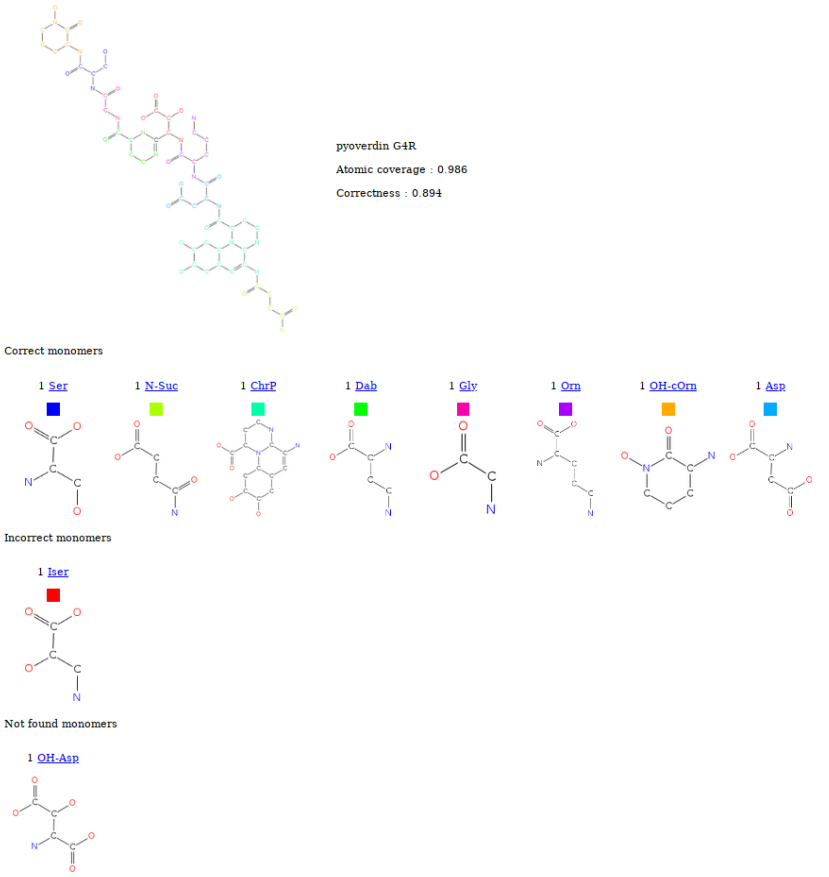
\includegraphics[width=0.9\textwidth]{images/pyoverdin G4R.png}
		\hspace{2cm}
		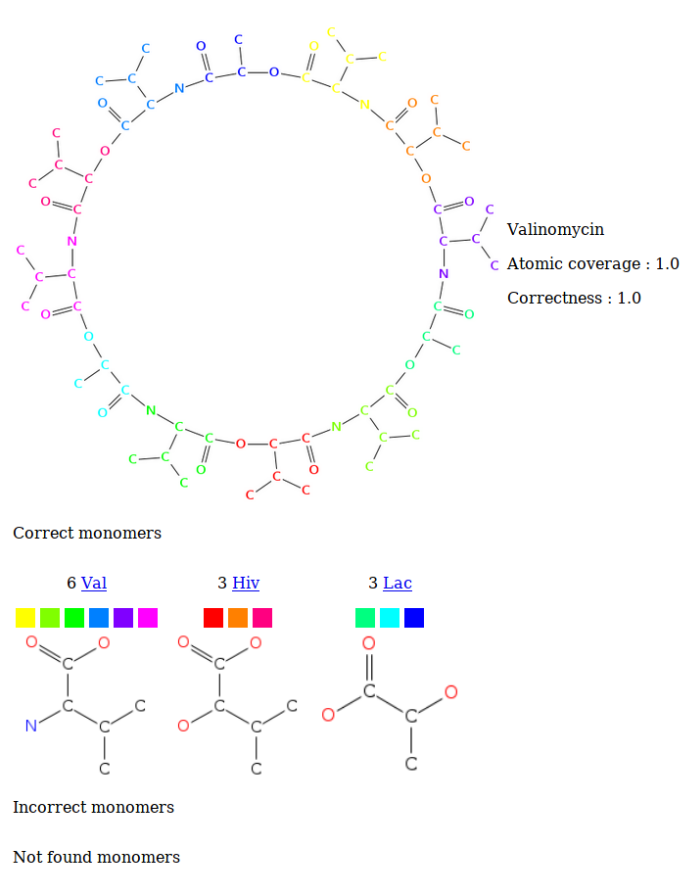
\includegraphics[width=0.5\textwidth]{images/Valinomycin.png}
	\end{figure}
	
	Les fichiers pris en entrée se trouvent dans le dossier $./data/$ et ceux de sortie dans $./build/results$. Pour changer le nom ou la position des fichiers pris en entrée ou ceux de sortie, il faut utiliser le paramètre $-D$ de ant, avec le nom de la  variable associée au fichier souhaité, puis lui donner le nouveau chemin et nom du fichier. Par exemple, si je souhaite changer le chemin pour le fichier $polymers.json$, initialement dans $./data/$, j'indique $ant$ $s2m$ -$Dexec.polymers="./directory1/polymeres.json"$ à la place de $ant$ $s2m$.
	
	\begin{figure}[H]
		\captionsetup{justification=centering}
		\centering
		\includegraphics[width=0.6\textwidth]{images/ants2m.png}
	\end{figure}
	\vspace{0.000000000001cm}
	\begin{figure}[H]
		\captionsetup{justification=centering}
		\centering
		\includegraphics[width=0.6\textwidth]{images/ants2m-D.png}
	\end{figure}
	
	rBAN propose quand à lui le choix du nom et du lieu des fichiers. L'utilisation de base prend en entrée un fichier de polymères dont on doit indiquer l'emplacement et le nom, ainsi que le nom du fichier de sortie. Ce dernier est un fichier $.json$ contenant :
	\begin{itemize}
		\item l'identifiant
		\item le Smiles
		\item la couverture atomique (coverage)
		\item la correctness
		\item la description des monomères qui le composent
	\end{itemize}

	Le fichier de polymères contient les informations suivantes:
	\begin{itemize}
		\item id
		\item nom
		\item smiles
	\end{itemize}
	
	Le fichier de sortie est composé pour chaque polymère :
	\begin{itemize}
		\item id
		\item Smiles
		\item couverture atomique (coverage)
		\item correctness
		\item les monomères le composant avec pour chacun :
		\begin{itemize}
			\item id
			\item cid
			\item codes
			\item noms
			\item Smiles
			\item masse
			\item boolean, s'il est nouveau
			\item boolean, s'il est identifié
		\end{itemize}
	\end{itemize}
	
	Pour que le programme génère les images des polymères, il faut saisir le paramètre -$imgs$ et pour que la banque de monomères soit une banque différente de Norine, il faut ajouter le paramètre -$monomersDB$ suivi du chemin et du nom fe la banque, au format $.json$.
	
	\begin{figure}[H]
		\captionsetup{justification=centering}
		\centering
		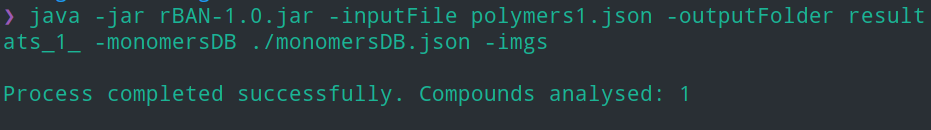
\includegraphics[width=0.6\textwidth]{images/java-jarrBAN-monoDB-imgs.png}
	\end{figure}
	\vspace{0.000000000001cm}
	\begin{figure}[H]
			\captionsetup{justification=centering}
			\centering
		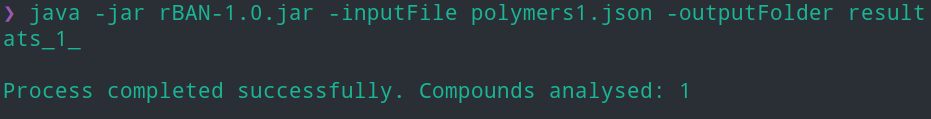
\includegraphics[width=0.6\textwidth]{images/java-jarrBAN.png}
	\end{figure}
	
	
	
	La couverture atomique correspond au taux auquel le polymère est recouvert par les monomères. Ainsi, les atomes en noir étant ceux n'appartenant à aucun monomère de la couverture, ils indiquent par leur présence que la couverture atomique est inférieur à 1.
	
	Les polymères Norine ont dans leur description un champ "graph" qui est le découpage en monomères du polymère. Ceci permet de vérifier le taux d'exactitude du découpage de Smiles-2Monomers et de rBAN. Ce taux est appelé Correctness dans les fichiers de sortie.
	
	La différence entre ces deux programmes réside dans leur stratégie de recherche. Smiles2-Monomers essaie dans un premier temps de positionner tout les monomères de la banque puis reconstitue au mieux le polymère à partir des monomères précédemment identifiés. La configuration rendue est celle dans laquelle il n'y a pas de chevauchement et dans laquelle le taux de couverture est le plus élevé. rBAN, quand à lui découpe les polymères en fonction des liaisons chimiques. Les morceaux sont comparés aux monomères de la banque pour déterminer à quel monomère le morceau correspond. S'il ne correspond à aucun monomère, il peut par exemple re-solidariser des morceaux voisins et de nouveau essayer d'identifier le monomère auquel il correspond.
	
	\chapter{Description des exemples traités}
	Le principal du travail a été réalisé en python, j'ai dû à un moment donné parcourir le code de Smiles2Monomers ainsi que le fichier $build.xml$.
	
	Le premier travail à réaliser a été de mettre en forme les banques de données récupérées de Norine.
	
	La deuxième étape a été le passage aux polymères de PubChem. Il a donc fallu récupérer, au début, les données sur le serveur REST de PubChem et également lancer les programmes  sur d'autres ordinatures que le mien, pour des raisons de performances. J'ai donc utilisé ceux du FIL(Formation en Informatique de Lille). Pour ce faire, j'ai appris à réaliser une connection $ssh$ avec un ordinateur, souvent le $a12p26$. Pour gérer et récupérer les fichiers, j'utilisais FileZilla pour que la gestion des fichiers et dossiers soit plus simple ; le tout passant par le VPN de l'université.
	
	Un premier script réalisait la conversion du fichier obtenu en un format accepté par les deux programmes puis deux autres scriptes en lançant plusieurs petits, chacun ne réalisant qu'une seule tâche. Le premier réalise le découpage du fichier contenant 500'000 polymères en \textit{n} fichiers, \textit{n} étant le nombre d'ordinateurs utilisés pour réaliser les calculs. Initialement, j'ai arbitrairement choisi de prendre \textit{n}=10. Vient ensuite le gros du calcul avec, au début, la récupération de \textit{m} polymères sur PubChem, la récupération des données utiles, le "nettoyage" des Smiles, le lancement de Smiles2Monomers et rBAN sur ces \textit{m} polymères, la copie des résultats de chacun et enfin de nouveau la même chose avec les \textit{m} polymères suivants. Pour pouvoir isoler plus facilement les polymères qui posent problème, \textit{m} a été fixé à 10, puis pour accélérer le temps de calcul, il a été placé à 1'000.
	
	La dernière étape fut enfin de remplacer les monomères de Norine par ceux de HELM, permettant ainsi de lancer les scripts pour faire tourner les programmes sur les données PubChem et HELM et en récupérer les résultats pour réaliser des statistiques sur la couverture atomique.
	
	Le plus difficile dans tout ce processus a été la gestion des versions, car je n'avais pas la même version d'ant chez moi que sur les ordinateurs du FIL, ce qui a engendré des erreurs quand je n'avais que des warnings quand je testais le tout sur mon ordinateur. Mais le plus difficile a surtout été le nettoyage des Smiles. Smiles2Monomers accepte plus de Smiles que rBAN. Il faut donc parvenir, en regardant un Smiles, à déterminer l'origine de l'erreur. Ainsi, plusieurs modifications ont été apportées aux Smiles :
	\begin{itemize}
		\item "\verb|.|" : Les Smiles contenant des points sont plusieurs polymères, il faut donc couper au niveau du point et traîter séparément chaque polymère (ex:
		\\"\verb|CC(C)(C)OC(=O)N[C@H](CC1=CC=C(C=C1)I)C(=O)=C.CC(C)(C)|\\\verb|OC(=O)N[C@@H](CC1=CC=C(C=C1)I)C(=O)=C|" devient \\"\verb|CC(C)(C)OC(=O)N[C@H](CC1=CC=C(C=C1)I)C(=O)=C|" et\\  "\verb|CC(C)(C)OC(=O)N[C@@H](CC1=CC=C(C=C1)I)C(=O)=C|" [ici, les deux polymères sont l'isomère l'un de l'autre]).
		
		\item "\verb|[14CH3]|" : Le carbone 14 ne doit plus être distingué des autres (ex : "\verb|CC(C)|\\\verb|[C@H]1C(=O)N([C@H](C(=O)O[C@@H](C(=O)N([C@H](C(=O)O|\\\verb|[C@@H](C(=O)N([C@H](C(=O)O1)CCCNC(=O)N)[14CH3])C(C)|\\\verb|C)CCCNC(=O)N)[14CH3])C(C)C)CCCNC(=O)N)[14CH3]|" devient \\"\verb|CC(C)[C@H]1C(=O)N([C@H](C(=O)O[C@@H](C(=O)N([C@H](C|\\\verb|(=O)O[C@@H](C(=O)N([C@H](C(=O)O1)CCCNC(=O)N))C(C)C)C|\\\verb|CCNC(=O)N))C(C)C)CCCNC(=O)N)|").
		
		\item "\verb|[H]|" et "\verb|[2H]|" : Les hydrogènes ne sont pas utiles et ceux entre crochets sont un problème, ainsi, on les enlève simplement.
		
		\item "\verb|[SeH]|" : Même problème que pour "\verb|[H]|" mais en plus, le symbole est en 2 lettres, il faut donc qu'il soit entre crochets, ce qui donne "\verb|[Se]|" à la place de "\verb|[SeH]|".
		
		\item "\verb|[nH]|" : De même que pour "\verb|[SeH]|" mais comme l'atome a un symbole en une seule lettre, on peut simplement ne garder que lui : "\verb|[nH]|" devient "\verb|n|".
		
		\item "\verb|[H:|\textbf{x}\verb|]|" : Avec \textbf{x} un chiffre, écriture HELM (Smiles apportant plus d'informations que le Smiles) n'est pas accepté par les programmes, on retire cette donnée.
		
		\item "\verb|[OH:|\textbf{x}\verb|]|" : Avec \textbf{x} un chiffre, même problème que \verb|[H:|\textbf{x}\verb|]| mais avec "\verb|O|" qui doit être conservé.
		
		\item "\verb|Se Si Cl Ca Br Na"|" : Les atomes dont le symbole est en plusieurs lettres doivent être mis entre crochets, ce qui donne "\verb|[Se] [Si] [Cl] [Ca] [Br] [Na]|".
		
		\item "\verb|/ \|" : Ces symboles signifient la présence d'une isomérie mais posent problème à rBAN, on les retire.
		
		\item "\verb|+ -|" : Les charges des ions sont à enlever une fois encore pour rBAN, sans oublier le nombre de charges s'il y en a plusieurs (ex : "\verb|[Ca2+]|" devient "\verb|[Ca]|")
		
		\item "\verb|cycles|" : Pour rBAN, s'il y a plus de 9 cycles, il y a un problème lié à la numérotation des cycles. Ils sont numérotés de 1 à 9, puis sont toujours 1 sauf s'il y en a deux qui se croisent, auquel cas le second est numéroté 2. Pour rBAN, chaque numéro de cycle doit être unique. Les numéros au dessus de 9 sont réservés aux atomes qui terminent 2 cycles ou en terminent un en en commençant un autre. Ainsi, ces polymères ne peuvent être traîtés en attendant de trouver une solution, ils sont retirés de la banque utilisée.
		
		\item "\verb|C2H7NO|" : La formule brute des molécules n'est pas acceptée par les programmes.
	\end{itemize}

	\chapter{Pseudo-Code}
	%\lstset{language=C}
	\begin{lstlisting}
		Coverage :
		0.0 -> 195
		0.1 -> 0
		0.2 -> 1
		0.3 -> 8
		0.4 -> 1699
		0.5 -> 315
		0.6 -> 2375
		0.7 -> 25427
		0.8 -> 139092
		0.9 -> 207199
		1.0 -> 126079
		NaN -> 14
	\end{lstlisting}
	
	Je remercie Madame Touzet de m'avoir accepté en stage dans son équipe.
	
	Je remercie Madame Pupin pour m'avoir encadrée et accompagnée tout au long de ce stage, particulièrement suite à la crise sanitaire du Covid-19.
	
	Je remercie Monsieur Noé pour son aide au sujet des connections avec les ordinateurs du FIL.
	
	Je remercie Clémentine Campart pour son aide et son temps.
	
	Je remercie enfin les enseignants responsables du FIL et du laboratoire qui ont permis que le stage soit maintenu, bien que réalisé en télé-travail.
	
	\chapter*{Conclusion}
	\pagenumbering{Alph}
	
	Smiles2Monomères a finalement été lancé sur 7 ordinateurs et les calcules ont été réalisés en 4heures environ.
	
	rBAN quand à lui à été lancé sur \textbf{n} ordinatuers et a fini en \textbf{h}heures.
	Ce dernier ne parvient pas à traiter tout les Smiles, on a donc supprimé ceux qui soit déclenchent une erreur, soit bouclent à l'infini.
	
	En plus des fichiers de sortie des deux programmes, des fichiers contenant les monomères et polymères modifiés et ceux supprimés ont été générés. Enfin, des statistiques ont été générées sur chaque fichier de sortie, contenant le nombre de polymères dont la couverture atomique est comprise entre 0.0 et 0.1, puis entre 0.1 et 0.2, ... le nombre de polymères dont la couverture atomique est égale à 1 et enfin la couverture égale à NaN (Not a Numbers).
	
	%\section{Résultats Smiles2Monomers}
	502404 polymères ont été traités. 
	Voici le contenu du fichier de statistiques de Smiles2Monomers :
	\lstset{language=Javascript}
	\begin{lstlisting}
	Coverage :
		0.0 -> 195
		0.1 -> 0
		0.2 -> 1
		0.3 -> 8
		0.4 -> 1699
		0.5 -> 315
		0.6 -> 2375
		0.7 -> 25427
		0.8 -> 139092
		0.9 -> 207199
		1.0 -> 126079
		NaN -> 14
	\end{lstlisting}
	\vspace{2cm}
	Cet histogramme présente ces données :
	\begin{figure}[H]
		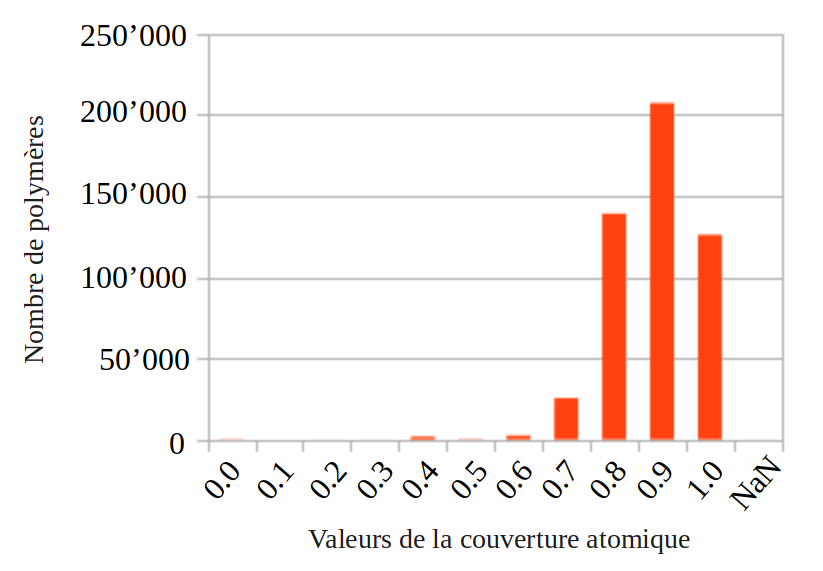
\includegraphics[width=0.8\textwidth]{./images/ACs2m.png}
	\end{figure}
	
	Cet histogramme nous permet de nous rendre compte que Smiles2Monomers parvient à traiter les peptider ribosomiques sans trop de problème. La majorité des polymères sont recouverts à plus de 70\% et le taux de couverture de la majorité des polymères est de 0.9.
	
	%\section{Résultats rBAN}
	
	
	
	\chapter*{Bilan personnel}
	
	Ce stage m'a permis d'apprendre de nouvelles choses en chimie, en biologie et en informatique, j'ai également réutilisé ce que j'avais fait et appris en Label Recherhce.
	
	Je n'ai pas tant découvert le monde du travail étant en télétravail, mais j'ai cependant appris à me débrouiller dans des situations dans lesquelles je ne m'étais jamais retrouvée, comme lors de ma découverte d'ant et lors des premières connections aux ordinateurs du FIL. J'ai toujours pu compter sur l'aide de Madame Pupin et ai été aidé par Monsieur Noé et une alternante de l'équipe, Clémentine Campart.
	
	Les réunions en début de chaque semaine et les rapports à mon tuteur universitaire m'ont donné un cadre et un rythme.
	
	Le sujet m'a vraiment passionnée et je suis sincèrement reconnaissante envers Madame Touzet de m'avoir acceptée en stage dans son équipe, ainsi que Madame Pupin de m'avoir encadrée, guidée, aidée et orientée tout au long de ce stage.
	
	
	
\end{document}